\subsection{Problem 3: Speech Recognition from Speech Spectrum}

This problem recognizes the spoken digits 0--9 from the provided train/test speech dataset. Each \texttt{.wav} file was converted into a $64 \times 64$ Mel spectrogram, then classified as an image using a CNN. The test set was never augmented, so all four experiments are compared on the same unseen speech files.

\subsubsection{Network and Input Representation}
The preprocessing pipeline loads each waveform, converts it to a 64-bin Mel spectrogram at 16 kHz, resizes it to $64 \times 64$, and normalizes the spectrogram. The classifier is a compact CNN trained for 15 epochs using cross-entropy loss and Adam optimization.

\subsubsection{Required Augmentation Experiments}
The assignment requires four runs: baseline, speech-domain augmentation, spectrum-image augmentation, and combined augmentation. Table~\ref{tab:prob3_results} summarizes the completed experiments.

\begin{table}[H]
    \centering
    \caption{Problem 3 speech recognition results}
    \label{tab:prob3_results}
    \begin{tabular}{|p{0.23\linewidth}|p{0.36\linewidth}|c|c|c|}
        \hline
        \textbf{Experiment} & \textbf{Augmentation Applied} & \textbf{Accuracy} & \textbf{Training Time} & \textbf{Testing Time} \\
        \hline
        (a) Baseline & None & 94.0\% & 28.01 s & 0.40 s \\
        \hline
        (b) Speech augmentation & Speed factor $0.97$ or $1.03$ and Gaussian waveform noise $\mathcal{N}(0,0.005)$ & 90.0\% & 38.61 s & 0.35 s \\
        \hline
        (c) Spectrum-image augmentation & Horizontal squeeze/expand by 3\% and Gaussian image noise & 93.0\% & 37.49 s & 0.42 s \\
        \hline
        (d) Combined augmentation & Speech augmentation plus spectrum-image augmentation & 89.7\% & 47.68 s & 0.41 s \\
        \hline
    \end{tabular}
\end{table}

\begin{figure}[H]
    \centering
    \begin{minipage}{0.48\linewidth}
        \centering
        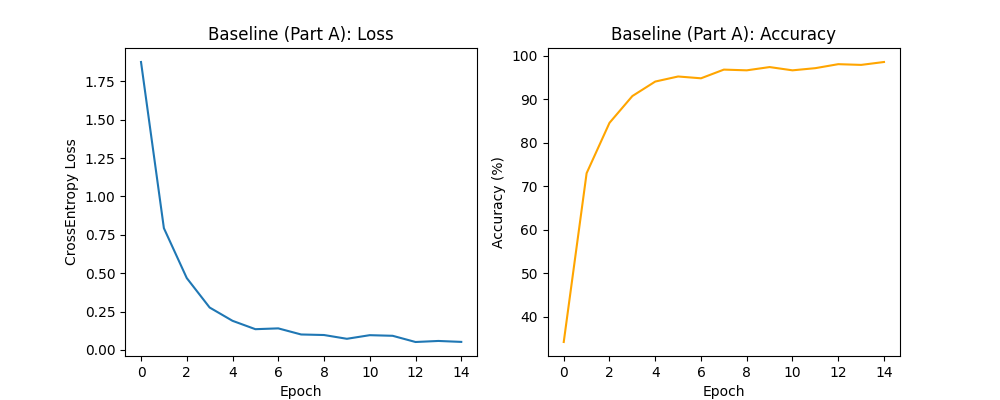
\includegraphics[width=\linewidth]{../Part1_Problem3_Speech/results/Baseline_Part_A_curve.png}

        {\small (a) Baseline}
    \end{minipage}
    \hfill
    \begin{minipage}{0.48\linewidth}
        \centering
        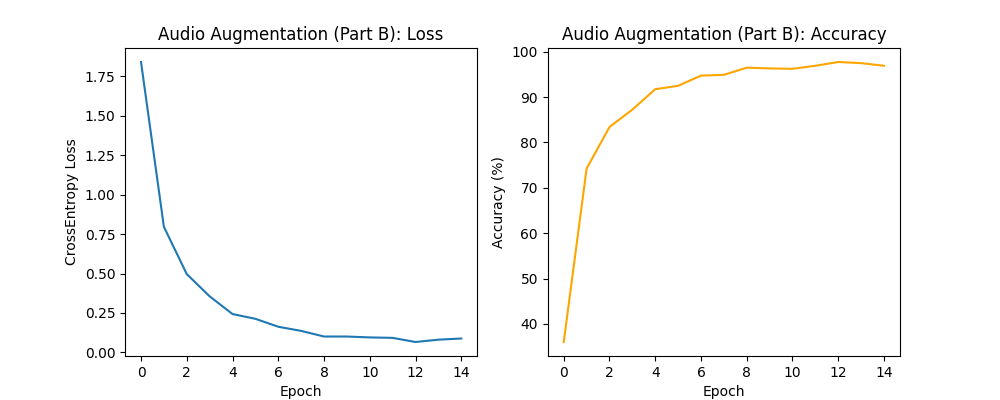
\includegraphics[width=\linewidth]{../Part1_Problem3_Speech/results/Audio_Augmentation_Part_B_curve.png}

        {\small (b) Speech augmentation}
    \end{minipage}

    \vspace{0.8em}

    \begin{minipage}{0.48\linewidth}
        \centering
        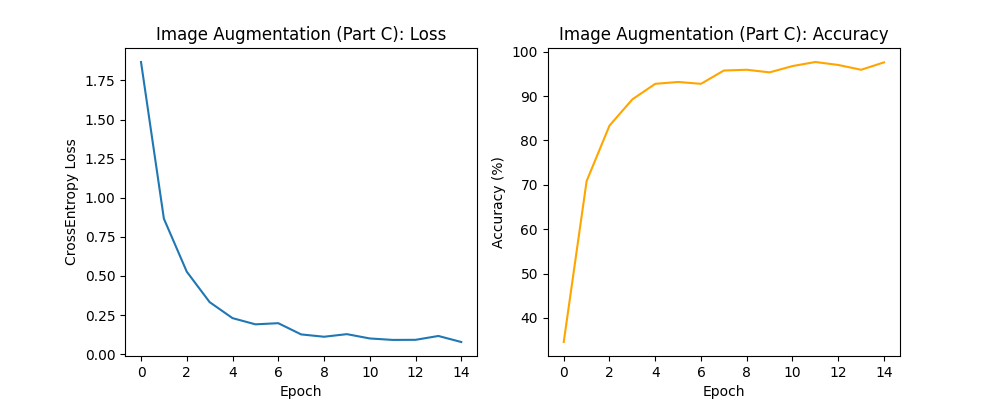
\includegraphics[width=\linewidth]{../Part1_Problem3_Speech/results/Image_Augmentation_Part_C_curve.png}

        {\small (c) Spectrum-image augmentation}
    \end{minipage}
    \hfill
    \begin{minipage}{0.48\linewidth}
        \centering
        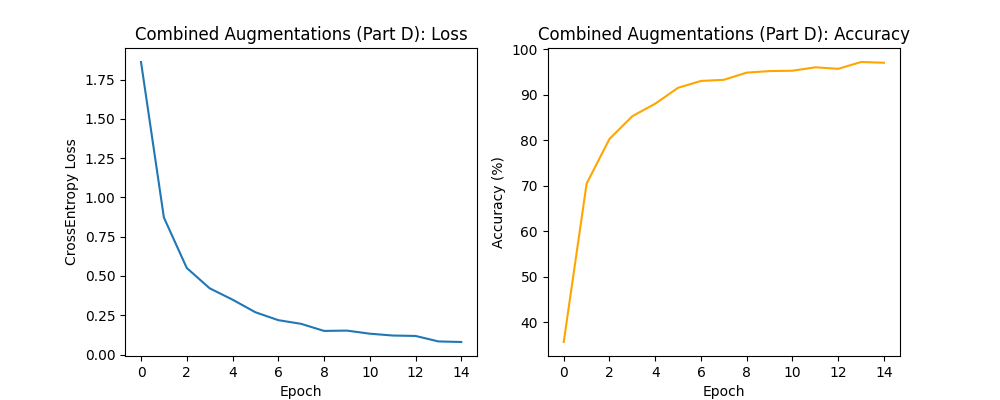
\includegraphics[width=\linewidth]{../Part1_Problem3_Speech/results/Combined_Augmentations_Part_D_curve.png}

        {\small (d) Combined augmentation}
    \end{minipage}
    \caption{Training curves for the four required speech-recognition experiments.}
    \label{fig:prob3_curves}
\end{figure}

\subsubsection{Discussion}
The baseline spectrogram CNN achieved the best result at $94.0\%$. Spectrum-image augmentation was close at $93.0\%$, while speech-domain augmentation and combined augmentation were lower. The drop suggests that the train/test split is already well represented by the baseline spectrogram features, and the added perturbations were stronger than necessary for this compact dataset. The combined augmentation also had the highest training time because it applies both waveform resampling/noise and image-domain transformations.
